\documentclass[12pt]{article}
\usepackage[utf8]{inputenc}

\usepackage[margin = 0.6in]{geometry}
\usepackage{amsmath}
\usepackage{amsfonts}
\usepackage{amssymb}
\usepackage{amsthm}
\usepackage{graphicx}
\usepackage{placeins}
\usepackage{enumitem}
\usepackage{dsfont}
\usepackage{booktabs}
\usepackage{subcaption}
\usepackage{pdflscape}

\newcommand{\N}{\mathbb{N}}
\newcommand{\Z}{\mathbb{Z}}
\newcommand{\R}{\mathbb{R}}
\newcommand{\E}{\mathbb{E}}
\newcommand{\Q}{\mathbb{Q}}
\newcommand{\de}{\mathrm{d}}
\newcommand{\one}{\mathds{1}}

\title{ECON 899b: Problem Set 3}
\author{Katherine Kwok\footnote{I collaborated with Anya Tarascina and Claire Kim on this assignment.}}
\date{December 2021}

\begin{document}

\maketitle
\noindent \textbf{Overview:} For this assignment, the goal is to use the BLP algorithm to solve an aggregate demand model with quality differentiation. In this case, we use data on the US car industry between 1985 to 2015. \\\\
\noindent \textbf{Program:} \\\\
The attached code files ``helper\_functions.jl" contains implements this declares the necessary functions and structs. And then ``main\_program.jl" uses the defined functions to implement the following steps:
\begin{enumerate}
	\item Use both (1) contraction mapping and (2) combined contraction mapping and Newton's method to invert the demand function for the paramter value $\lambda_p = 0.6$ and the first year in the sample (1985).
	\item Find the parameter value $\lambda_p \in [0, 1]$ that minimizes the GMM objective function using 2SLS weighting matrix.
	\item Implement 2-step GMM with the minimum $\lambda_p$ from the previous step, using BFGS minimization routine.
\end{enumerate}
\noindent \textbf{Results:} \\\\
For the first step, Figures \ref{fixed_point_norm_evolution} and \ref{newton_norm_evolution} shows the evolution of the norm between the log of market share and log of predicted shares. As expected, the method using only contraction mapping takes double the number of iterations compared to the combined method. Since the Newton method makes step adjustments while accounting for the curvature of the function, it converges more quickly.\\\\
For the second step, Figure \ref{gmm_obj_func} displays the evolution of the GMM objective function value over the paramter grid between 0 and 1. We find that the GMM objective function is minimized around 0.6.\\\\
Finally, the two-step GMM method estimates the optimal $\lambda_p = 0.6194$. Table \ref{tab1} summarizes the associated variable estimates, including price and other car characteristics.

\begin{figure}[!htbp]
	\centering
	\caption{Evolution of Norm for Contraction Mapping Method}
	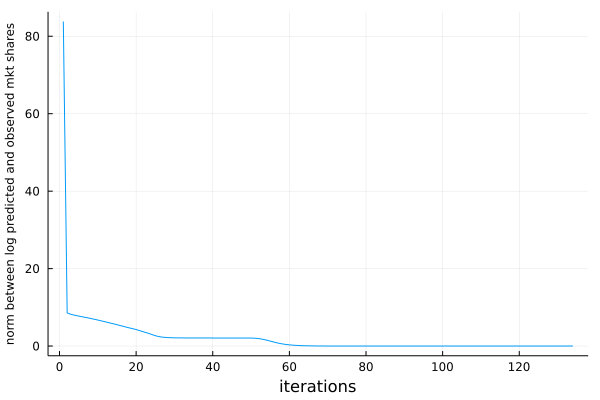
\includegraphics[width = 0.8\textwidth]{fixed_point_norm_evolution.png}
	\label{fixed_point_norm_evolution}
\end{figure}

\begin{figure}[!htbp]
	\centering
	\caption{Evolution of Norm for Combined Contraction Mapping Method and Newton}
	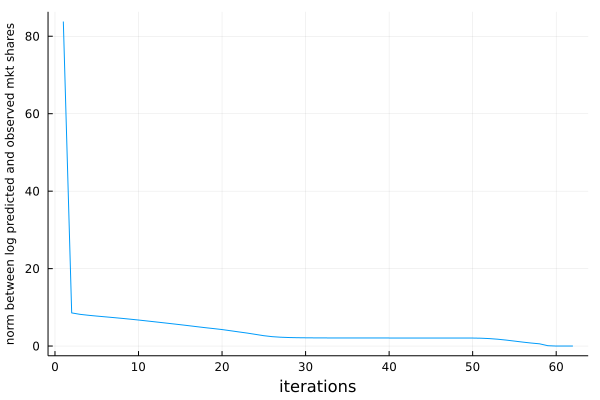
\includegraphics[width = 0.8\textwidth]{newton_norm_evolution.png}
	\label{newton_norm_evolution}
\end{figure}

\begin{figure}[!htbp]
	\centering
	\caption{GMM objective function over $\lambda_p \in [0,1]$}
	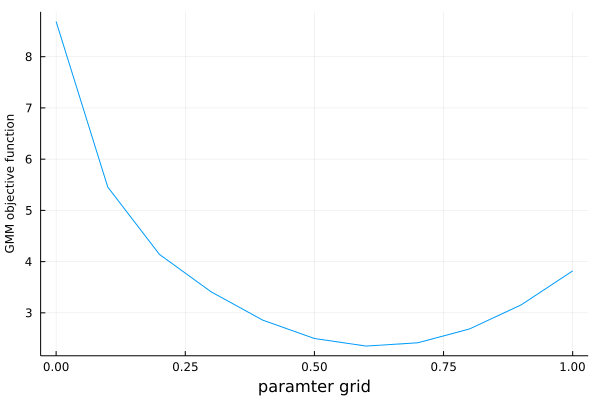
\includegraphics[width = 0.8\textwidth]{gmm_obj_func.png}
	\label{gmm_obj_func}
\end{figure}

% Please add the following required packages to your document preamble:
% \usepackage{booktabs}
\begin{table}[!htbp]
  \caption{Variable Estimates}
  \label{tab1}
  \small \centering
\begin{tabular}{@{}ll@{}}
\toprule
variables       & estimates \\ \midrule
price           & -3.264    \\
dpm             & -0.199    \\
hp2wt           & 0.302     \\
size            & 4.498     \\
turbo           & 0.533     \\
trans           & -0.436    \\
Year\_1986      & -0.033    \\
Year\_1987      & -0.139    \\
Year\_1988      & -0.049    \\
Year\_1989      & 0.003     \\
Year\_1990      & -0.357    \\
Year\_1991      & -0.644    \\
Year\_1992      & -0.653    \\
Year\_1993      & -0.478    \\
Year\_1994      & -0.121    \\
Year\_1995      & -0.013    \\
Year\_1996      & -0.035    \\
Year\_1997      & 0.053     \\
Year\_1998      & 0.122     \\
Year\_1999      & 0.393     \\
Year\_2000      & 0.559     \\
Year\_2001      & 0.117     \\
Year\_2002      & 0.176     \\
Year\_2003      & 0.158     \\
\bottomrule
\end{tabular}
\begin{tabular}{@{}ll@{}}
\toprule
variables       & estimates \\ \midrule
Year\_2004      & 0.084     \\
Year\_2005      & 0.15      \\
Year\_2006      & -0.23     \\
Year\_2007      & -0.641    \\
Year\_2008      & -1.159    \\
Year\_2009      & -2.654    \\
Year\_2010      & -2.21     \\
Year\_2011      & -1.759    \\
Year\_2012      & -1.26     \\
Year\_2013      & -1.005    \\
Year\_2014      & -0.795    \\
Year\_2015      & -0.823    \\
model\_class\_2 & -0.788    \\
model\_class\_3 & 0.392     \\
model\_class\_4 & -0.092    \\
model\_class\_5 & -0.786    \\
cyl\_2          & -1.311    \\
cyl\_4          & -0.852    \\
cyl\_6          & 0.151     \\
cyl\_8          & 0.284     \\
drive\_2        & 0.403     \\
drive\_3        & 0.26      \\
Intercept       & -2.423    \\
\\
\bottomrule
\end{tabular}
\end{table}


\end{document}
